\documentclass[14pt,a4paper]{memoir}
\usepackage{listings}
\usepackage[framemethod=tikz]{mdframed}
\usepackage{graphicx}
\usepackage{textcomp}
\usepackage{lipsum}
\usepackage{gensymb}
\usepackage{amsmath}
\usepackage{hyperref}
\graphicspath{ {./images/} }
\usepackage{xepersian}
\settextfont{XB Zar}
\setlatintextfont{Times New Roman}
\deflatinfont\mono[Scale=.9]{Courier New}




\definecolor{mycolor}{rgb}{0.122, 0.435, 0.698}

\newmdenv[innerlinewidth=0.5pt, roundcorner=4pt,linecolor=mycolor,innerleftmargin=6pt,
innerrightmargin=6pt,innertopmargin=6pt,innerbottommargin=6pt]{mybox}


\newmdenv[innerlinewidth=0.5pt, roundcorner=4pt,linecolor=mycolor,innerleftmargin=6pt,
innerrightmargin=6pt,innertopmargin=6pt,innerbottommargin=6pt]{tip}




\begin{document}
		
		
		
\frontmatter
	
	\title{ بازی سازی و برنامه نویسی خلاقانه پایه}
	\author{چوبک بیدپا}
	\date{}
	\clearpage\maketitle
	\thispagestyle{empty}
	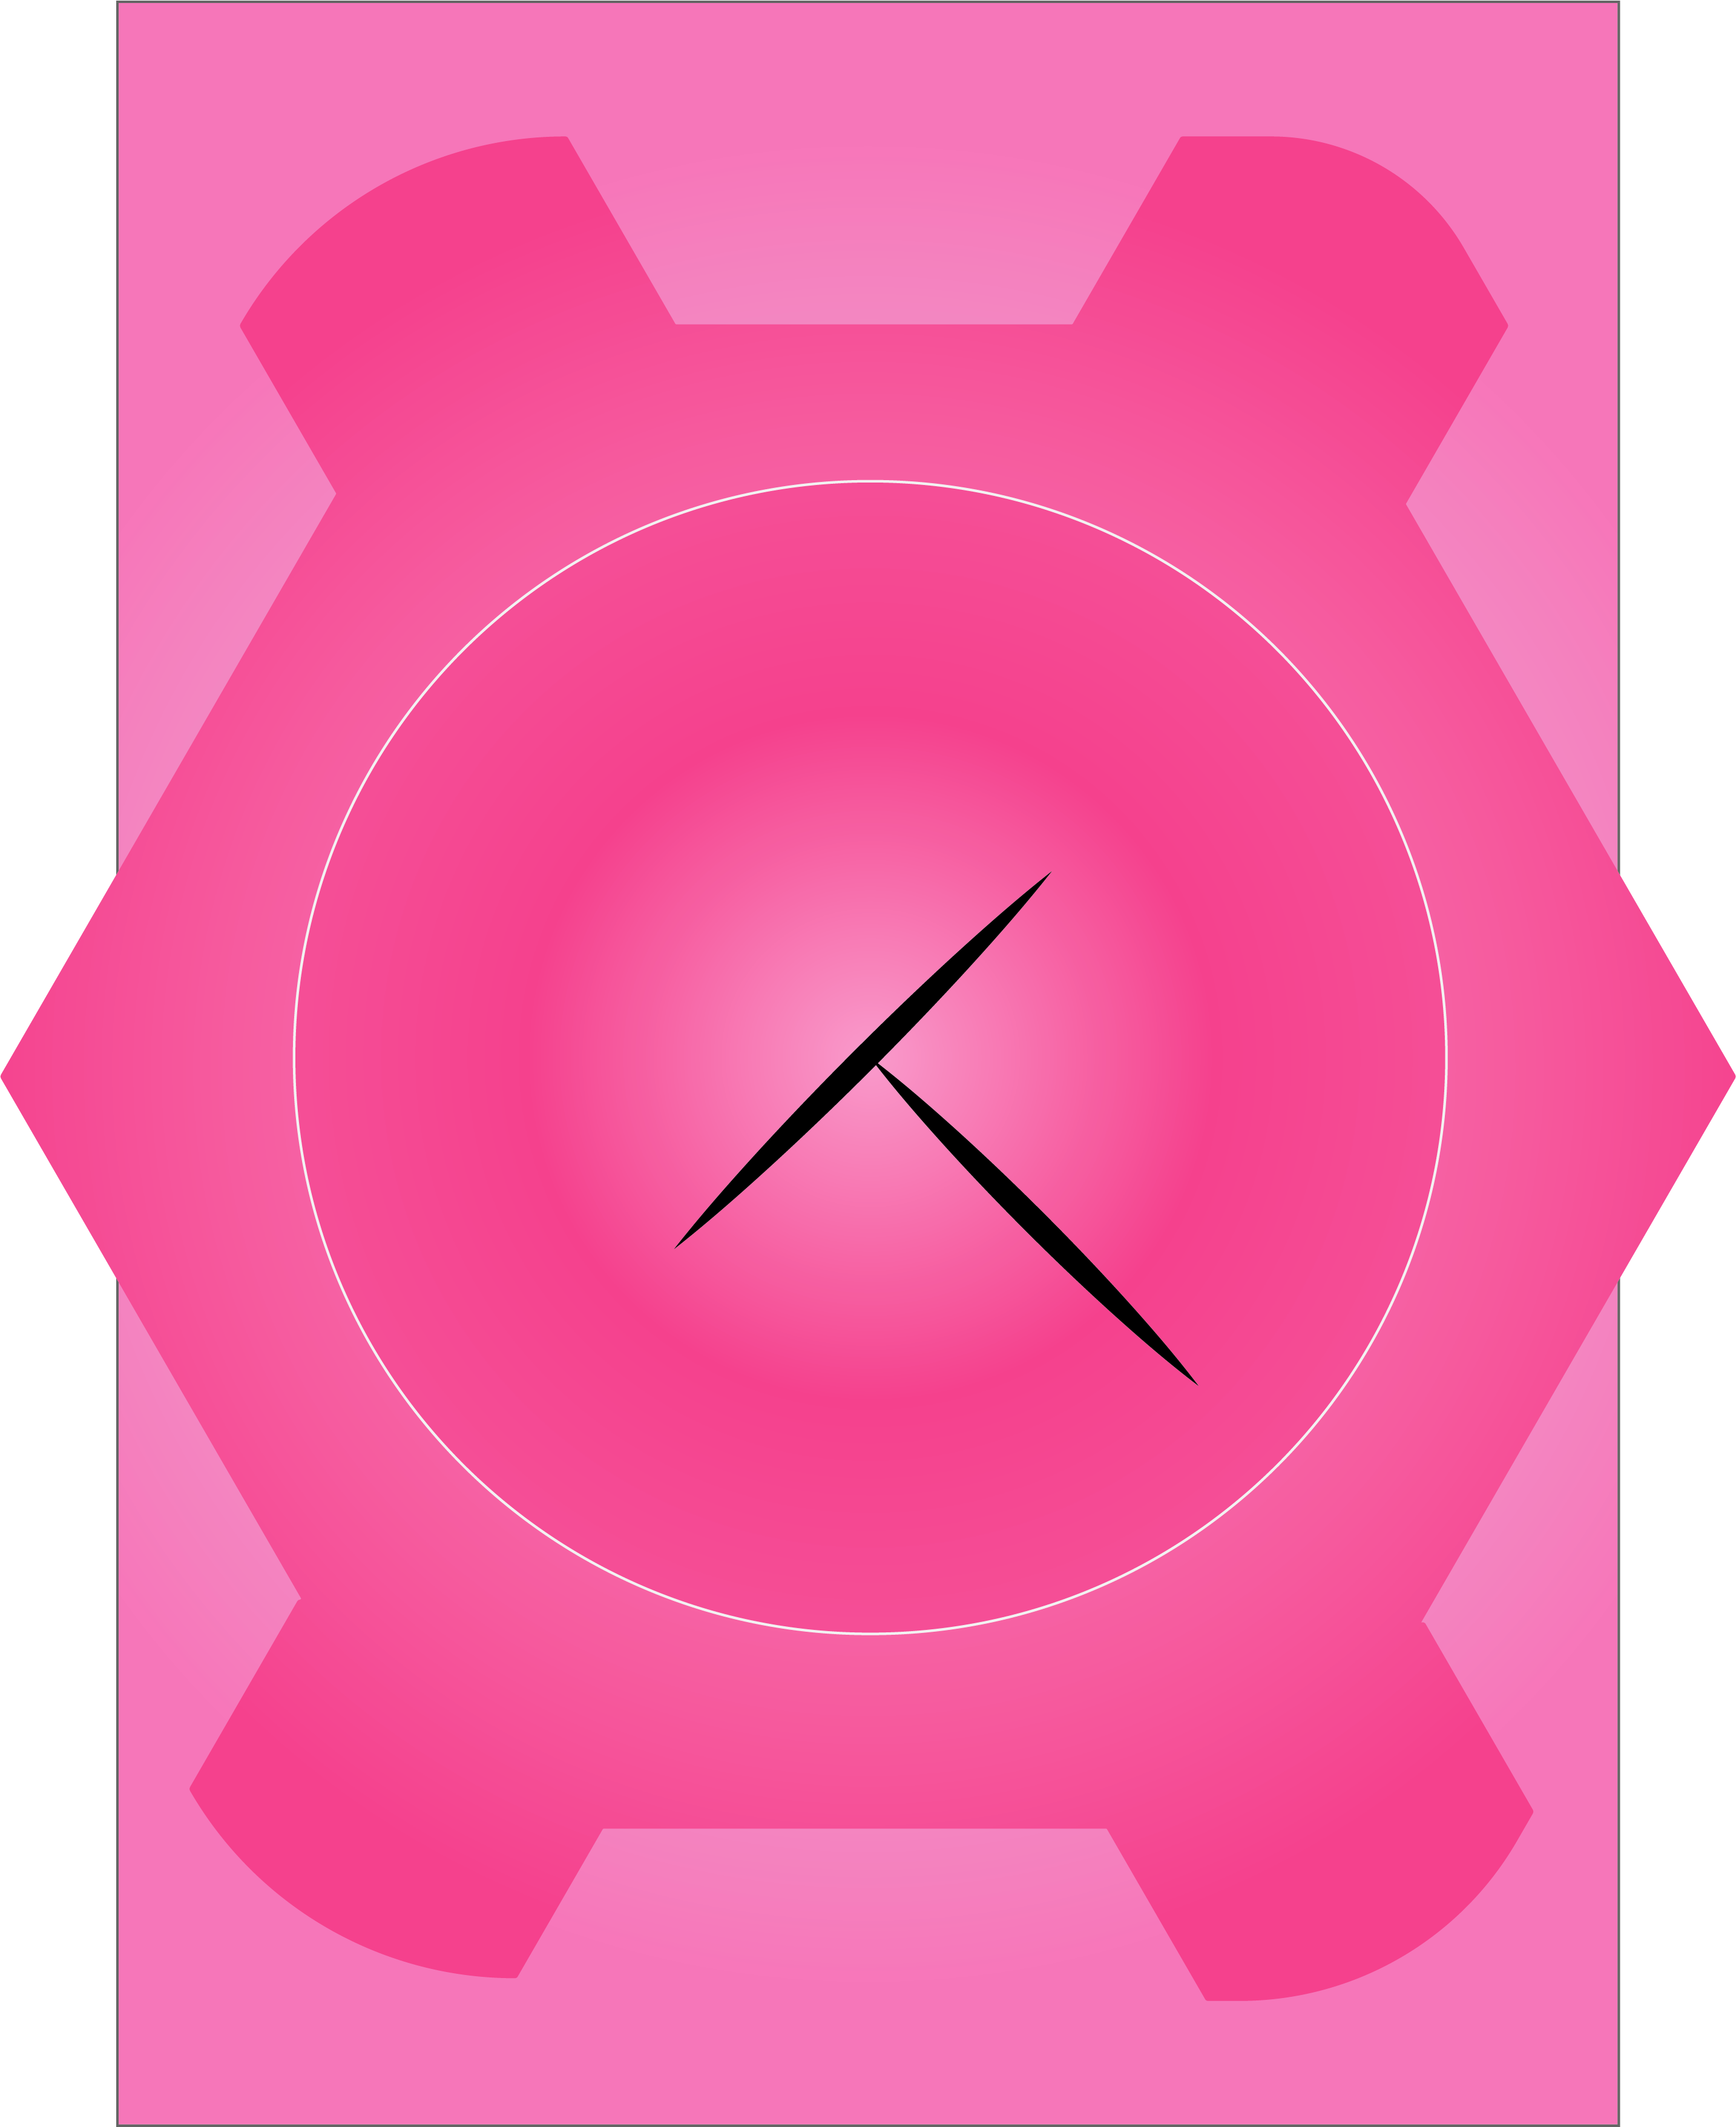
\includegraphics[scale=0.6]{Cover}	
	\newpage
	
		

	
	\begin{mybox}
		\begin{center} عرضه شده تحت لیسانس MIT\\ 1397
				\vfill
				نویسنده: چوبک بیدپا
				\vfill
				سال عرضه: 1397
				\vfill
				کاملا رایگان \vfill
				جهت برقراری ارتباط با چوبک بیدپا از ایمیل \url{chubakbidpaa@riseup.net} استفاده نمایید.
	\end{center}	


	\end{mybox}
 
 
	 \vfill
	 
	 به خاطر اینکه بخش قابل توجهی ازین کتاب، از آموزشهایی که تحت لیسانس \lr{Creative Commons}، MIT و GPL عرضه شده اند استفاده میکند، استفاده ، تکثیر و آموزش این کتاب، به شرط نام بردن نویسنده یعنی شخص حقیقیِ چوبک بیدپا، آزاد میباشد.
	 
	 توجه داشته باشید که فایلهایی که همراه کتاب به فروش گذاشته شده اند، غیرقابل تکثیر بوده، و آپلود آنها توسط شخص حقیق چوبک بیدپا قابل قبول میباشد.
	 
	 تحت قوانین Transference، شما جهت استفاده از بخشهای این کتاب که توسط افراد دیگر نگاشته شده اند احتیاجی به اجازه از آنها ندارید.
	 
	 در آخر، قابل توجه باشد که این کتاب یک پروژه ی اشتیاقی \footnote{\lr{Passion Project}} می باشد، و نه پروژه ای که برای به دست آوردن پول نوشته شده است. برای همین، مرام را به جای آورید و آنرا در جای دیگر آپلود نکنید.
	 
	 لطفا فایلهایی که همراه کتاب خریده اید نیز جایی کپی نکنید. قیمت فایلها با توجه به استطاعت خوانندگان، با الگوریتمی پیچیده\footnote{با بیشتر شدن تعداد خریدارها، قیمت کاهش میابد.} تعیین شده است. برای همین همه میتوانند آن را بخرند. آپلود فایلهای کتاب در جای دیگر، پایرسی حساب میشود و از لحاظ اخلاقی، کاریست نپسندیده.
	 
	 اما تکثیر خود کتاب با ذکر منبع آزاد است.
	  
	 \textbf{نکته:} کدهای کتاب در فایل خریداری شده حی و حاظر آماده ی کپی میباشد.
	 
	 
	 
	 \chapter*{قراردادهای کتاب}
	 
	 \begin{enumerate}
	 	\item  بخشهای کتاب: این کتاب به دو بخش برنامه نویسی خلاقانه\footnote{\lr{Creative Programming}}، و بازی سازی تقسیم شده است.
	 	\item  نکته: نکته های خاص کتاب در به این صورت مشخص شده اند:
	 		
	 	
	 				\begin{tip}
	 					نکته اینجاست که....
	 				\end{tip}
	 
	 \item استفاده از فایلها: اگر فایلی لازم باشد، نام و آدرس آن در فایل زیپ دانلود شده نوشته خواهد شد.
	 \item یو آر الها به صورت \url{https://google.com} نوشته خواهند شد.
	 \item متن پررنگ: وقتی لازم است روی کلمه ای تاکید کنم، یا کلمه جدید است و قبلا استفاده نشده، از \textbf{متن پررنگ} استفاده خواهد کرد.
	 \item کد: کدهایی لازمه به صورت زیر نوشته خواهند شد.
	 
	 
	\begin{latin}
	\mono{	\begin{lstlisting}
		for i:=maxint to 0 do
		begin
		{ do nothing }
		end;
		Write('Case insensitive ');
		Write('Pascal keywords.');
		\end{lstlisting}}
	
	\end{latin}
	 
	\end{enumerate}
	 
	 
	 \tableofcontents
	 \mainmatter
	 
	 \chapter{چند کلمه با خواننده} \label{foreword}

	«آزادی خود را گرامی بدارید، وگرنه آنرا از دست میدهید.»
	امروزه، جبهه های مختلفی هستند که بر آزادی اطلاعات عقیده دارند. یکی از آنها نهاد گنو\footnote{GNU} است که کِرنل سیستم عامل لینِکس\footnote{Linux} را در دست دارد. دیگری مازیلاست\footnote{Mozilla}، که مرورگر فایرفاکس\footnote{Firefox} را منتشر کرده است. 
	
	من به شخصه معتقدم آژادی اطلاعات از آزادی بیان مهمتر است، چون اگر اطلاعات را برای خود نگه داریم، کمتر کسی راههای اشاعه ی آزادی بیان را یاد خواهد گرفت، یا اصلا خواهد دانست که آژادی بیان چه هست. 
	
	این کتاب نه تنها بر پایه ی عقیده به آزادی اطلاعات\footnote{\lr{Freedom of Information}} مجانی است، بلکه یکی از دلایل مجانی بودن آن اینست که تمام آن مال من نیست، بلکه، حدود 30\% این کتاب، ترجمه ی آموزشهای اینترنت، با اجازه از صاحبان آنهاست. 20\% این کتاب، از داکیومنتشنهای رسمی برداشته شده  و 50 درصد باقی را خودم نوشته ام.
	
	شاید برایتان سوال باشد چرا این کتاب را نگاشت کرده ام. دلیل اصلی آن اینست که دلیلی داشته باشم تا برنامه نویسی را ادامه دهم. بعضی ها پروژه مینویسند، بعضی ها کتاب مینویسند. من در لفافه ی کتاب، پروژه مینوسم. تمام پروژه های کتاب اریجینال بوده، و فایلهایی که همراه کتاب خریده اید، کار من هستند.
	
	دلیل دیگری که این کتاب را نوشته ام، اینست که کتاب های بازی سازی به زبان فارسی کم هستند، و کمتر کسی در ایران از برنامه نویسی خلاقانه خبر دارد. سعی من درینست که با نوشتن در مورد این دو دیسیپلین دوست داشتنی، فرهنگ آنها را در کشور اشاعه بدهم.
	
	از سابقه ام در برنامه نویسی و بازی سازی بگویم. من از شانزده سالگی  \(الان 25 سال دارم \) کم و بیش در برنامه نویسی، و گهگاهی ساخت بازی، فعال بوده ام. مانند خیلی ها از نرم افزار \lr{Game Maker} کارم را شروع کردم \(درین کتاب از گیم میکر حرفی نخواهیم زد. نمیگویم انجین بدی است، میگویم اصلا انجین نیست!\) و با آن چندین بازی مانند تتریس، بریک اوت و... ساختم. من چندین بازی تحت اسکی مانند بلک جک نیز نوشته ام. من زبانهای سی پلاس پلاس، پایتان، و سی را میدانم و با زبان اسکریپت نویسی چندین نرم افزار آشنایی دارم. درضمن نمره ی تافلم در 17 سالگی 95 بوده پس به ترجمه ام اعتماد کنید.
	
	سابقه ی من در برنامه نویسی خلاقانه کمتر است. دو سال پیش بود که با نرم افزار افتر افکتس\footnote{\lr{After Effects}} آشنا شدم و به صرافت نوشتن پلاگین برایش افتادم، و طی این امر، با کتابخانه ی Cinder برای سی پلاس پلاس آشنا شدم. و از آنجا بود که با زبان Processing و شیدر ها آشنا گردیدم. الان تسلط کافی برای آموزش پایه ی شیدرها و زبانها و کتابخانه های برنامه نویسی خلاقانه دارم.
	
	بگذارید در مورد چارچوب کتاب کمی صحبت کنم. در این کتاب، دو بخش داریم، برنامه نویسی خلاقانه، و بازی سازی که به دو بخش Asset و برنامه نویسی تقسیم میشود. در بخش اَسِت سعی شده با استفاده از برنامه های مختلف، ساخت اسپرایت، تایل، اسپرایت شیت، تایل شیت، عکس پس زمینه، مدل سازی سه بعدی، و تکسچر و متریال \(که به بخش اول ربط دارد\) را آموزش دهم. در بخش برنامه نویسی کتابخانه ی Arcade پایتان، کتابخانه ی SFML سی پلاس پلاس، و انجین Godot \(گَدو\) آموزش داده خواهد شد. اگر قرصت شد، آموزشی کوتاه برای ساخت انجین خودتان را خواهم نوشت.
	
	قبل از هرچیزی دو چیز باید یادآوری شود: برنامه نویسی، و ریاضی. من زیاد در مورد این دو کانسپت حرف نمیزنم، چون وظیفه ی خود خواننده است که این دو را از قبل یاد داشته باشد، اما فقط در حد یادآوری، در مورد این دو حرف خواهم زد.
	 
	 من تازه نوشتن این کتاب را شروع کرده بودم و همین الان برای من موهبتی بوده است، چون باعث شد لِیتِک را یاد بگیرم و مطمئنم در طول کتاب، من بیشتر از شما خواهم آموخت! و آیا اینچنین نیست که همه، برای یادگیری، درس میدهند؟ هر کلمه ای که یاد میدهی، دو کلمه می آموزی. و این یک موهبت است.
	 
	 
	 در آخر، در این دنیای پر هیر و گیر، اگر پَشِنی دارید که به شما آرامش میدهد، نیکوست. و اگر این کتاب برای پیدا کردن این پَشِن کمک میکند، خوشحالم.
	 
	 \begin{flushleft}
	 	چوبک بیدپا
	 	مشهد - 1397
	 \end{flushleft}
	 
	 
	 
	 \chapter{نگاهی کوتاه به ریاضی لازمه}\label{math}
	 \section{توابع}\label{functions}

یک تابع\textbf{\footnote{Function} به صورت زیر نشان داده میشود:
\[y = f(x)\]}

وظیفه ی یک تابع، تغییر عدد داده شده بر اساس قوانین داده شده است. به این قانون، تابع میگویید. مثلا تابع \(f(x) = x^2\) که به آن تابع مربع می گویند، وظیفه اش بردن عدد به توان دو است. به عکس تابع، تابع \textbf{معکوس}\footnote{Inverse} میگویند و به صورت زیر نشان داده میشود:

\[y = f(x)^{-1}\]

مثلا معکوس تابع مربع، تابع ریشه دو یعنی $ f(x) = \sqrt{x} $ میباشد. میتوان دو تابع را با هم به صورت $ f(g(x)) $ ترکیب کرد که به آن تابع مرکب میگویند. از دیگر عملیاتها عبارت است از:

\[ (f + g)(x) = f(x) + g(x) \]
\[ (f - g)(x) = f(x) - g(x) \]
\[ (f * g)(x) = f(x) * g(x) \]
\[ (\frac{f}{g})(x) = \frac{f(x)}{g(x)} \]

به تمام اعدادی که تابع میپذیرد، \textbf{دامنه}\footnote{Domain}، و تمام اعدادی که تابع خارج میکند، \textbf{برد}\footnote{Range} خوانده میشود. دامنه ی یک تابع را ما تعیین میکنیم، اما برد آن را خود تابع تعیین میکند.

در آخر، بگذارید بگویم که تابع مانند یک ماشین است. ورودی آن $ x $ و خروجی آن $ f(x) $ است. در برنامه نویسی از توابع استفاده ی زیادی میشود. در بخش برنامه نویسی خواهید خواند.

\section{بردارها}\label{vector}

اگر فضای دوبعدی را به دو بخش نقاط افقی و نقاط عمودی تقسییم کنیم، \textbf{بردار}\footnote{Vector} خطی است که چهار نقطه را به هم وصل میکند.

\includegraphics*[scale=0.3]{Vector} 

بردار را به صورت زیر نشان میدهند:

\[ \vec{V} = (x_1, y_1) + (x_2, y_2) \]
	 
	 صفحه ی مختصات را به این صورت میکشیم: \vfill
	 \begin{center}
	 	\includegraphics*[scale = 1]{coordinate_system}
	 \end{center}
	 
	 که به آن \textbf{دستگاه مختصات دکارتی}\footnote{\lr{Carthesian Coordinate System}} میگویند. در دستگاه مختصات دکارتی، دو محور $ X $ و $ Y $ به ترتیب محور افقی و عمودی ما را تشکیل می دهند. ما مختصات یک نقطه را در پرانتز به صورت $ (X, Y) $ نشان میدهیم. همانطور که گفته شد، خطی که دو نقطه را به هم وط کند، بردار نام دارد.
	 
	 در جبر خطی، بردار را به صورت:
	 
	 \[\vec{V} = \begin{pmatrix}
	 X \\ Y
	 \end{pmatrix}
	 \] 
	 
	 نشان داده میشود و نقطه ی اول آن، مسقط الرأس دستگاه مختصات یعنی $ (0, 0) $ میباشد. 
	 
	 \begin{center}
	 	 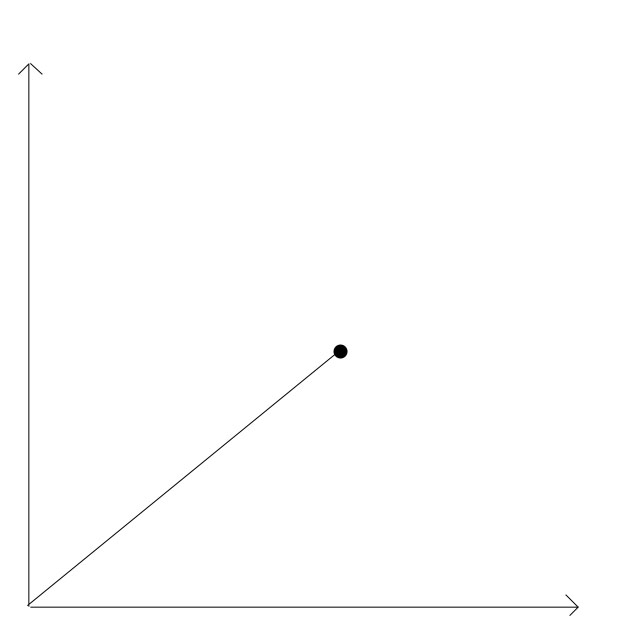
\includegraphics[scale=0.9]{LinAlgVec}
	 \end{center}
	
	به برداری که مختصات افقی، یا عمودی آن، یک باشد بردار واحد میگویند. بردار واحد افقی را $ \vec{i} $ و بردار افقی عمودی را $ \vec{j} $ میگویند. بردار ها را میتوان به صورت مضربی از بردار واحد نشان داد مثلا بردار $ \vec{V} = \begin{pmatrix}
	X \\ Y
	\end{pmatrix}$ را میتوان به صورت $ X\vec{i} + Y\vec{j} $ نشان داد. 
	
	
	
	
یک بردار دارای دو خصیصه می باشد. \textbf{جهت}\footnote{Direction} و \textbf{مقدار}\footnote{Magnitude}. که به صورت زیر نشان داده میشود:

	
		 \begin{center}
		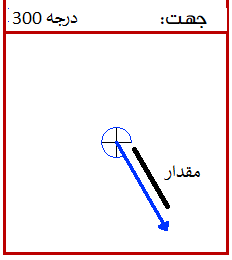
\includegraphics[scale=1]{DirMag}
	\end{center}

برای به دست آوردن مقدار بردار ازین فرمول استفاده میکنیم:
\[ |\vec{V}| =  \sqrt{x^2 + y^2} \]
	
	
	
	 
	 دو بردار را میتوان به صورت زیر جمع کرد:
	 
	 
	 	 \begin{center}
	 	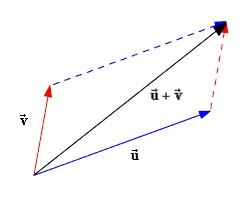
\includegraphics[scale=1]{VectorAdd}
	 \end{center}
 
 و به این صورت تفریق کرد:
  
 \begin{center}
 	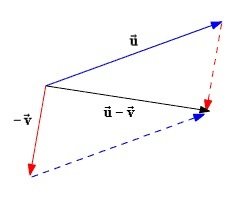
\includegraphics[scale=1]{VectorSubtract}
 \end{center}
 
	 
	 
	 اما دو نوع ضرب برداری داریم. \textbf{ضرب تقطه ای}\footnote{\lr{Dot Product}} و \textbf{ضرب صلیبی}\footnote{\lr{Cross Product}}. قبل ازین که پیش بروید، قسمت مثلثات \(\ref{trig}\) را بخوانید. فرض کنید دو بردار به صورت زیر هستند:
	 
	 
	  \begin{center}
	 	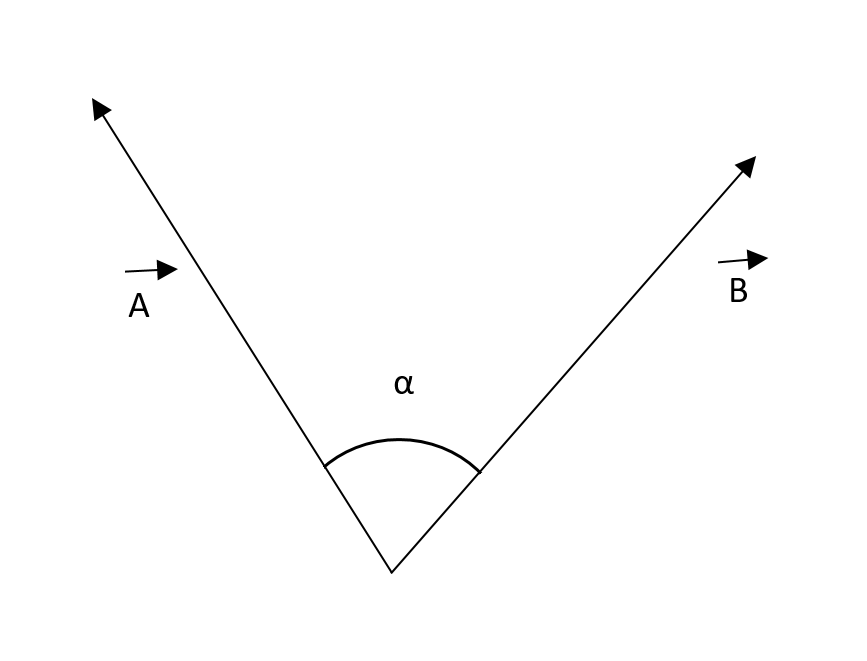
\includegraphics[scale=0.3]{Product}
	 \end{center}
	 
	 
	 ضرب نقطه ای به صورت زیر تعریف میشود:
	 
	 \[ \vec{A}.\vec{B} = |A||B|\cos \alpha \]
	 
	 و ضرب صلیبی ازین فرمول استفاده میکنیم.
	 \[ \vec{A} \times \vec{B} = |A||B|\sin \alpha \vec{n} \]
	 
	 
	 که  $\vec{n} $ برداری واحد عمود بر دو بردار است. برای به دست آوردن $\vec{n}$ کافیست از انگستان وسط، اشاره، و شصت خود استفاده کنید. انگشت شصت شما، همواره بردار واحد عمود است، که مضربی از ضرب صلیبی دو بردار می باشد.
	 
	 
	 \section{مثلثات}\label{trig}
	 
	 مثلثات بحثیست پیپیده. و من نیز ریاضیدان نیستم پس به کمی در مورد این مبجث قناعت میکنیم.  قبل از هرچیزی، بگذارید در مورد \textbf{دستگاه مختصات قطبی}\footnote{\lr{Polar Coordinate System}} حرف بزنم. دستگاه مختصات قطبی، مانند دستگاه مختصات دکارتی، دارای دو محور عمودی و افقی است. اما در این دستگاه مختصات، ما یک نقطه را، عوض $ X $ و $ Y $ توسط یک زاویه $ \alpha $ و یک بردار شعاع $ \vec{r} $ نشان میدهیم:
	 
	 
	 
	 	  \begin{center}
	 	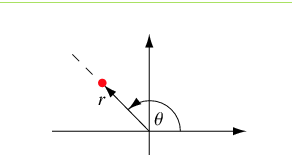
\includegraphics[scale=1]{Polar}
	 \end{center}
 
 در برنامه نویسی خلاقانه، دستگاه مختصات قطبی کاربردهای زیادی دارد. اما در کامپیوتر، \textbf{پیکسلها}\footnote{در مورد پیکسلها به وفور حرف خواهم زد.} در دستگاه مختصات دکارتی قرار دارند. حلال مشکلات ما، مثلثات است.
 یک دایره ی واحد را در دستگاه مختصات  قطبی کنید که شعاعش 1 میباشد:
  \begin{center}
 	\includegraphics[scale=1]{UnitCIrcle}
 \end{center}

اگر زاویه ی $   30\degree   $ را انتخاب کرده و یک مثلث قائم الزاویه دور آن بکشیم:


	   \begin{center}
	 	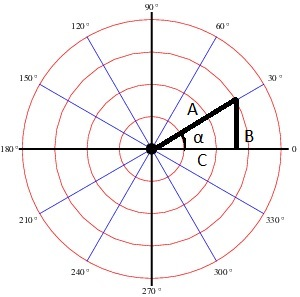
\includegraphics[scale=1]{ThirtyDegrees}
	 \end{center}
	 
	 سینوس و کسینوس زاویه 30 درجه که اینجا $ \alpha $ نامیده میشود، به صورت زیر تعریف میگردد:
	 \[ \sin \alpha = \frac{\text{مقابل}}{\text{وتر}} \]
	 
	 و:
	 
	 \[ \cos \alpha = \frac{\text{مجاور}}{\text{وتر}} \]
	 
	 همچنین تانژانت و کتانژانت به صورت زیر تعریف میشوند:
	 
	  \[ \tan \alpha = \frac{\sin \alpha}{\cos \alpha} \]
	  
	  
	  و 
	  \[ \cot \alpha = \frac{\cos \alpha}{\sin \alpha} \]
	  
	  
	  درجه، تنها واحد اندازه گیری زاویه نیست. واحد دیگر، \textbf{رادیان}\footnote{Radians} نام دارد. یک زاویه در رادیان، بین $ 0 $ و$   2\Pi $ قرار دارد. ارزش $ \Pi $ حدود $ 3.1415926535 $ است. ما برای کار با پیکسلها، ارقام اعشار بیشتر ازین نیز نیازمندیم. برای تبدیل درجه به رادیان:
	  \[ n\degree \times 	  \frac{\pi}{180} \]
	  
	  , و بالعکس:
	  
	  \[ n \space rad \times 	  \frac{180}{\pi} \]
	  
	  
	  
	  
	  توابع مثلثاتی توسط \textbf{هویتهای مثلثاتی}\footnote{\lr{Trigonometric Identities}} به هم ربط داده میشوند. بعضی ازین هویتها عبارتند از:
	  
	  \[ \sin^2 \alpha + \cos^2 \alpha = 1 \]
	  \[ \sin(-\alpha) = -\sin\alpha \]
	  \[ \cos(-\alpha) = \cos(\alpha) \]
	  \[ \sin(\alpha\pm\beta) = \sin\alpha\cos\beta \pm\cos\alpha sin\beta \]
	  \[ \cos(\alpha\pm\beta) = \cos\alpha\cos\beta\pm\sin\alpha\sin\beta \]
	 
	 
	 اینها تقریبا تمام سرفصهلایی هستند که شما برای این کتاب لازم دارید. توجه کنید، این کتاب، نه برنامه نویسی خلاقانه و بازی سازی کلی.
	 
	 \section{ماتریسها}\label{matrix}
	 
	 به آرایه هایی از اعداد که به صورت n سطر و m ستون به نمایش در می آیند.، \textbf{ماتریس}\footnote{Matrix} میگویند. یک ماتریس را به این صورت نشان میدهند:
	 \[ M_{m, n} = \begin{bmatrix}
	  a_{1,1} & a_{1,2} & \cdots & a_{1,n} \\
	 a_{2,1} & a_{2,2} & \cdots & a_{2,n} \\
	 \vdots  & \vdots  & \ddots & \vdots  \\
	 a_{m,1} & a_{m,2} & \cdots & a_{m,n}
	 \end{bmatrix} \]
	 
	 
	 در ساخت بازیهای کامپیوتری و برنامه نویسی خلاقانه ما بیشتر نیاز به ماتریسهای $ 2\times2 $، $ 3\times3 $  و $ 4\times 4$ داریم.
	 
	 جمع و تفریق ماتریسها به این صورت انجام میشود:
	 
	 \[ M_{m, n}\pm N_{m, n} = \begin{bmatrix}
	 m_{1, 1} \pm n_{1, 1} && m_{1, 2} \pm n_{1, 2} && \cdots &&  m_{1, n} \pm n_{1, n} \\
	 m_{2, 1} \pm n_{2, 1} && m_{2, 2} \pm n_{2, 2} && \cdots &&  m_{2, n} \pm n_{2, n} \\
	 \vdots  && \vdots  && \ddots && \vdots \\
	 m_{n, 1} \pm n_{n, 1} && m_{n, 2} \pm n_{n, 2} && \cdots &&  m_{n, n} \pm n_{n, n}
	 	
	 \end{bmatrix} \]
	 
	 ضرب ماتریسها به این روش صورت میپذیرد که، هر سطر با یک ستون. پس تا سطرها و ستونهای دو ماتریس با هم مساوی نباشند، ضرب صورت نمیپذیرد. 
	 
	
	 	{\fontsize{8}{10}\selectfont  \[ M_{1, n} \times N_{m, 1} = \begin{bmatrix}
	 		m_{1, 1} && m_{1, 2} && \cdots && m_{1, m}
	 		\end{bmatrix} \times \begin{bmatrix}
	 		n_{1, 1} \\
	 		n_{2, 1} \\
	 		\vdots \\
	 		n_{n, 1}
	 		\end{bmatrix} = (m_{1, 1} \times n_{1, 1}) + (m_{1, 2} \times n_{2, 1}) + \cdots + (m_{1, n} + n_{m, 1}) \]
	 	}
	 
	

یکی دیگر از عملیتهای ماتریسی، \textbf{دترمینان}\footnote{Determinant} است. برای احتساب دترمینان ماتریسهای بزرگتر از  $ 3\times3 $الگوریتمهای زیادی مانند \textbf{دیکامپوزیشن}\footnote{Decomposition} وجود دارد که خود آن توسط افراد مختلفی در طول سالها بهسازی گشته اند، اما راه ساده ای برای به دست آوردن دترمینان $ 2\times2 $ وجود دارد که به شرح زیر است:

\[ A = \begin{bmatrix}
A && B\\ 
C && D
\end{bmatrix} \]
\[ |A| = AD - BC \]
	 
	 به $ I_{n} $ ماتریس \textbf{هویت} \footnote{Identity} میگویند و مثلا $ I_3 $ به صورت زیر تعری میشود:
	 
	 \[ I_{3} = \begin{bmatrix}
	 1 && 0 && 0 \\
	 0 && 1 && 0 \\
	 0 && 0 && 1
	 \end{bmatrix} \]
	 
	 ما در برنامه نویسی خلاقانه و بازی سازی از ماتریسها استفاده های زیادی خواهیم برد.
	 
	 \section{قائمیت در فضای سه بعدی}\label{r3}
	 
	 
	 ما در بخش بردار دیدیم که دستگاه مختصات دکارتی شامل دو محور عمودی و افقی است. اما همیشه اینگونه نیست، بلکه، میتوان با اظافه کردن یک بردار اضافه که نام آن $ Z $ است به دستگاه سه بعدی دست پیدا کنیم. این دستگاه را به صورت $ \mathbf{R^3} $ نشان میدهند و در تصویر زیر میتوانید محور $ Z $ را مشاهده کنید:
	  
	 
	 
	 \begin{center}
	 	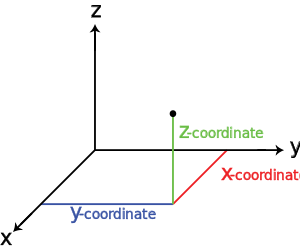
\includegraphics[scale=1]{R3}
	 \end{center}
	 
	 توجه کنید که در بعضی از نرم افزارها جای $  Y $ با $ Z $ عوض میشود.
	 
	یک بردار را در فضای $ R^3 $ به صورت زیر نشان میدهیم:
	
	\[ \vec{V} = \begin{pmatrix}
	X\\Y\\Z
	\end{pmatrix} \]
	 
	 
	 همه ی قوانین $ R^2 $ برای  $ R^3 $ برقرار است. مثلا به بردار واحد محور $ Z $، $ \vec{k} $ میگویند. غرض از این بخش، اینست که \textbf{قائمیت}\footnote{ Orthogonality} در فضای سه بعدی را معرفی کنم. زیرا برای بازیهای دو و نیم بعدی، دوربین باید قائم بر فضای $ R^3 $ باشد.
	 
	 
	 \begin{center}
	 	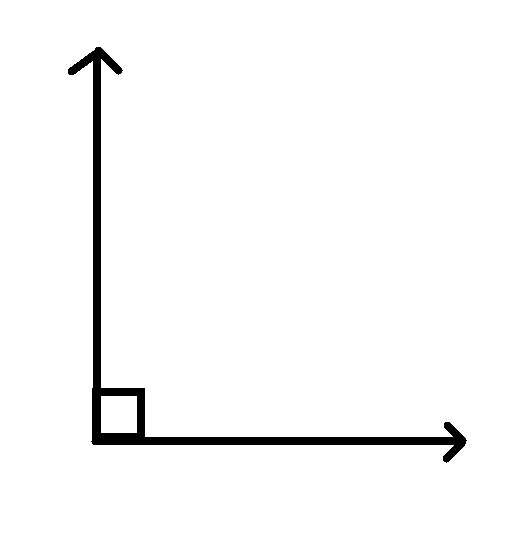
\includegraphics[scale=1]{Orthogonal}
	 \end{center}
	 در کل، دو بردار وقتی بر هم قائمند که حاصلضرب نقطه ای آندو، صفر باشد:
	 \[ \vec{A} \text{قائم است بر } \vec{B} \text{اکر و تنها اگر} \vec{A}.\vec{B} = 0 \]
	 
	 
	 
	 اگر فرمول ضرب نقطه ای یادتان باشد، و در اینترنت کسینوس 90 را خوانده باشید، میدانید که:
	 
	 
	 
	 \[ \vec{A}.\vec{B} = |A||B|\cos \alpha \]
	 
	 و $ \ cos(90)  = 0$
	 پس:
	 
	 \[ |A||B|\cos (90) = 0 \ \]
	 
	 
\section{پایان فصل ریاضی}\label{mathend}

کلید یادگرفتن ریاضی یک چیز است: $  \text{تمرین}^n  $! یادتان نرود که حافظه، چیزیست فرَار، و هر لحظه ممکن است همین چیزهای کمی که از بنده ی حفیر آموخته اید، که مطمئنم برای بیشتر شما یک یادآوری ساده و کوتاه بوده، و برای خیل عظیمی از شما فوت آب بوده، و فقط یک لیست است، سریع از حافظه ی شما رخت برمیبندند. تمرین کنید، نوت برداری کنید، و یادتان نرود که روم را در یک روز نساخته اند. این ضرب المثال را چندین بار در طول کتاب تکرار خواهم کرد. یادگیری طول میکشد. و یادتان نرود که هیچکس استعداد چیزی را ندارد، و همه چیز با تمرین میسر میشود.

در فصل بعد، در مورد برنامه نویسی، زبان پایتان و \lr{C++} حرف خواهیم زد.
	 
	   
	 \chapter{نگاهی کوتاه به برنامه نویسی}\label{programming}
	 
	 درین فصل نگاهی کوتاه می اندازیم به \textbf{برنامه نویسی}\footnote{Programming}. ابتدا به دو \textbf{پَرَدایم}\footnote{Paradigm} برنامه نویسی \textbf{فانکشنال}\footnote{Functional} و \textbf{شیء گرا}\footnote{\lr{Object Oriented Programming}}. و بعد \textbf{پیچیدگی زمانی}\footnote{\lr{Time Complexity}} را توضیح خواهیم داد. بعد از آن، نگاهی می اندازیم به \textbf{سینتکسِ}\footnote{به دستور زبانی یک زبان برنامه نویسی Syntax گفته میشود.} زبان \textbf{پایتان}\footnote{Python} و \textbf{\lr{C++}}.
	 
\section{برنامه نویسی فانکشنال}\label{functional}

از بین تمام روشها، یا به عبارتی، پَرَدایمهای برنامه نویسی، برنامه نوسی فانکشنال یا \textit{تابعی} ساده ترین، و پر مصرف ترین آنهاست. اکثر اشخاصی که برنامه نویسی را شروع میکنند، از برنامه نویسی فانکشنال شروع میکنند. زبانهای قدیمی مانند \textbf{فورترن}\footnote{FORTRAN}	و \textbf{لیسپ}\footnote{Lisp} همه فانکشنال هستند. 

با توابع در فصل ریاضی آشنا شدیم. توابع کامپیوتری نیز با توابع ریاضی فرق زیادی ندارد، همه ی آنها یک ماشین هستند که ورودی را به خروجی تبدیل میکنند. یک تابع، مجموعه ای از \textbf{دستورات}\footnote{Instructions} است که \textbf{پارامتر}\footnote{Parameter} داده شده را با تغییرات، باز میگردانند. این تغییرات میتواند عملیاتهای جمع و تفری، ضرب و تقسیم، باقیمانده، و یا تغییر نوع پارامتر مثلا از عدد صحیح به عدد حقیقی، و یا هرچیز دیگری باشد. برای اجرای تابع، آنرا \textbf{میخوانیم}\footnote{Call} و به پارامتری که به آن میدهیم، \textbf{آرگومان}\footnote{Argument} میگوییم.

اینستراکشن سِت زیر را در نظر بگیرید:

\begin{enumerate}
	\item عدد $ n $ را بگیر.
	\item برای $ n $ بار، $ n $ را ضربدر $n - 1$ کن.
	\item جواب را برگردان.

\end{enumerate}

به این تابع، تابع \textbf{فاکتوریل}\footnote{Factorial} میگویند. توابع زیادی هستند، پیچیده و ساده، مهم اینجاست که از آنها درست استفاده کنید. 
بعضی از توابع، پارامتر قبول نمیکنند. بعضی از توابع، ارزشی را باز نمی گردانند. به این نوع از توابع \textbf{ووید}\footnote{Void} میگویند. بعضی از زبانها، \textbf{تایپ ثابت}\footnote{\lr{Statically Typed}} هستند و باید نوع ارزشهای باز گرداننده را مشخص کرد. \lr{C++} یکی ازین نوع زبانهاست. بعضی از زبانها \textbf{تایپ دینامیک}\footnote{\lr{Dynamically Typed}} هستند و لازم نیست نوع ارزش بازگرداننده را در آنها مشخص کرد. پایتان یکی ازین زبانهاست. هردو زبان پایتان و \lr{C++} هم فانکشنال هستند، هم شیء گرا. در مورد پَرَدایم شیء گرا در بخش بعد صحبت خواهیم کرد. 
هرزبان مقداری تابع از پیش تغیین شده دارد، اما بقیه ی تابع ها را خودتان باید تعیین کنید. اینکه در چه زمانی باید تابع تعیین کرد، قانون طلایی اینست که هرگاه دیدید عملی را دارید بیشتر از یک بار انجام میدهید، وقت تعیین کردن یک تابع است. 
همه ی زبانها دارای \textbf{کتابخانه}\footnote{Library} هایی هستند که شامل توابع و کلاسها \(\ref{oop}\) و دیگر کدهایی هستند که به برنامه نویس کمک میکنند خود را تکرار نکند.
 
	 
	\textbf{خود را تکرار نکنید.}\footnote{\lr{DRY - Don't Repeat Yourself}}
	
	قانون پلاتینیوم برنامه نویسی، اینست. هرگز چیزی که در یک کتابخانه موجود است را ننویسید. مثلا عوض اینکه در زبان \textbf{جاوا}\footnote{Java} عوض نوشتن صدها خط کد برای به دست آوردن یک تابع ماتریس، میتوان از کتابخانه ی JAMA استفاده کرد.
	
	
	
	
	
	
	 
	 \section{برنامه نویسی شیء گرا}\label{oop}
	 
	 
	 
	 
	 
	 
	 
	 
	 
	 
	 
	 
	 
	 
	 
	 
	 
	 
	 
\end{document}